\subsection{Descripción general}
El diagrama de Máquinas de Estados Finitos tiene como objetivo principal mostrar el detalle de ciertos procesos dinámicos que no se pueden apreciar correctamente en el Diagrama de Actividad.

\subsection{Relación con otros modelos}


\newpage
\subsection{Vistas}

El primer diagrama que mostraremos es el funcionamiento de las actualizaciones durante la etapa de seguimiento de un proyecto. Para simplificar, no consideramos en el escenario la posibilidad de que cambie el PM del proyecto, o cancele el proveedor, ya que son dos posibilidades que están detalladas en el Diagrama de Actividad.

La variable $limite_dias$ mencionada, responde al intervalo de actualizaciones durante el cual debe haber almenos una actualización. Este limite es particular de cada proyecto y lo configura el Gerente al momento de la creación del mismo.

\begin{center}
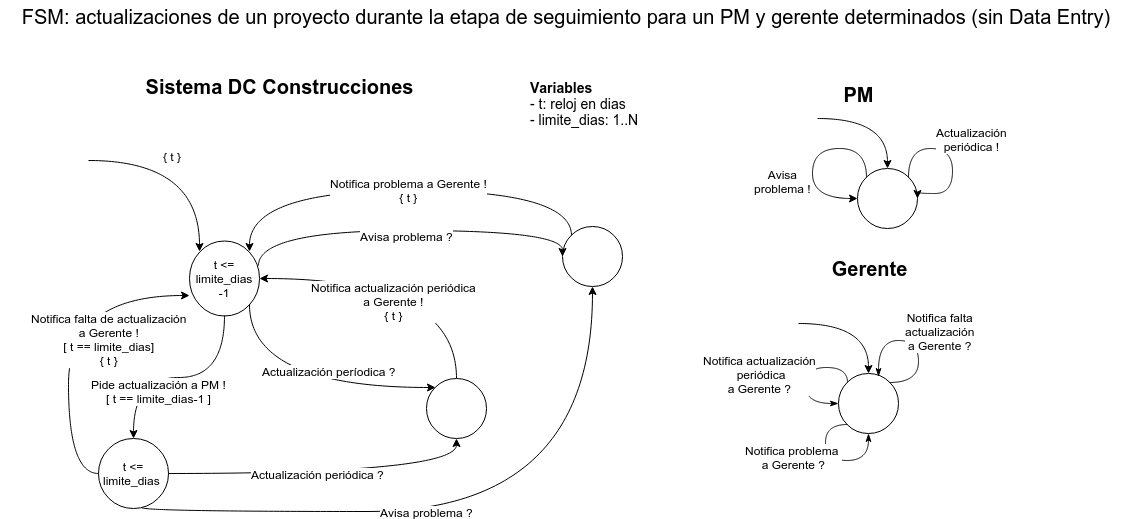
\includegraphics[scale=0.5, angle=90]{imagenes/FSM1.png}
\end{center}

\newpage
El segundo diagrama que mostraremos es el detalle del proceso mediante el cual el Cliente y el Gerente acuerdan el presupuesto a través del Sistema.

\begin{center}
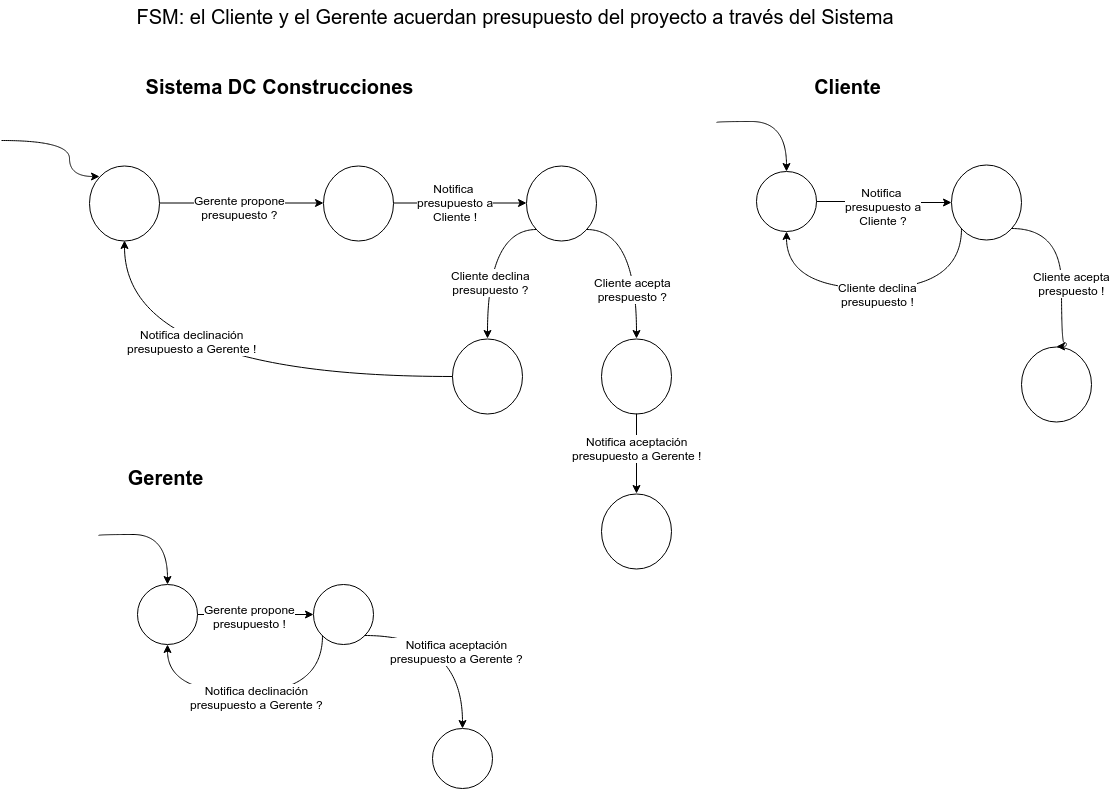
\includegraphics[scale=0.5, angle=90]{imagenes/FSM2.png}
\end{center}

\newpage
El tercer diagrama que mostraremos es el detalle del proceso mediante el cual el Cliente y el PM acuerdan el alcance del proyecto a través del Sistema.

\begin{center}
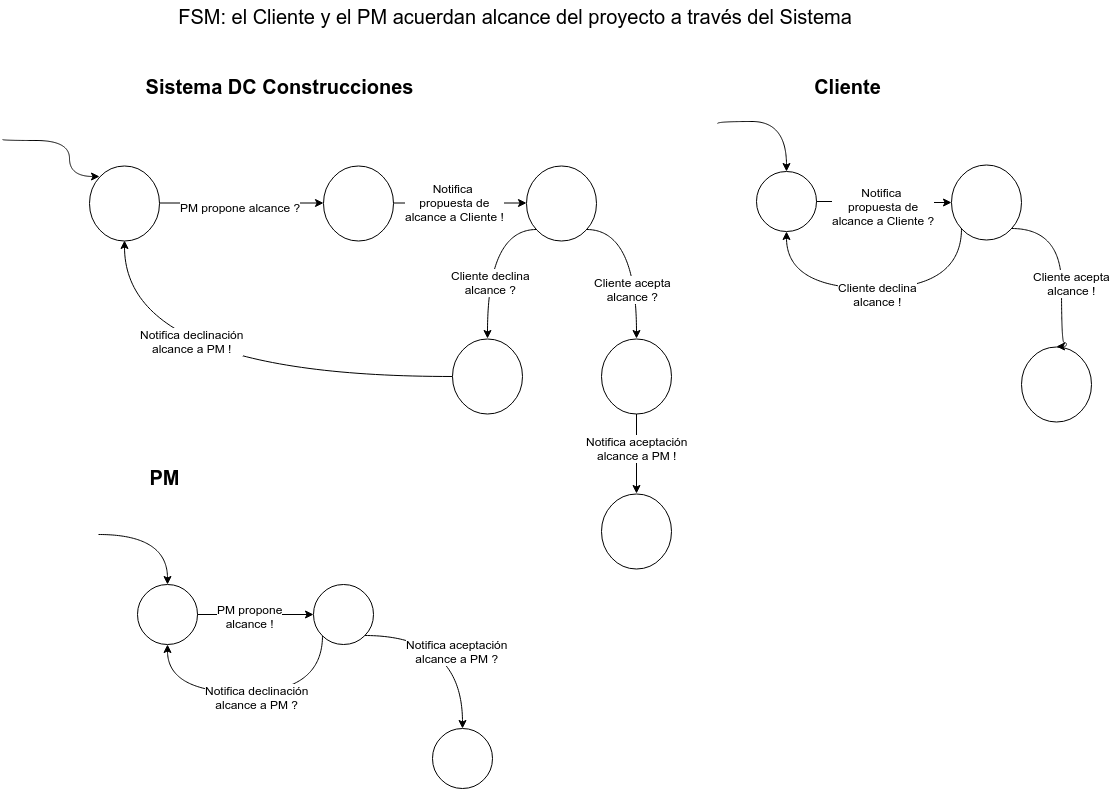
\includegraphics[scale=0.5, angle=90]{imagenes/FSM3.png}
\end{center}
